% !TEX root = ../partial-sdm.tex

Performance matters --- and has always mattered. If an experiment takes a few seconds, there is no point arguing whether we should try it. If it takes a few hours, maybe we should think first. If it takes a few days, it is more important to make a good plan. As SDM consumes a lot of both processor and memory resources, some experiments may take a long time.

Each scan a 1,000-bits SDM with 1,000,000 hard-locations executes $10^9$ bit compares through $10^9/64 = 15,625,000$ XORs and calls to the built-in popcount. So, 10,000 writes execute $10^{13}$ bit compares, while a 6-iterative reading executes $6 \cdot 10^{12}$ bit compares. The heatmap of Figure \ref{fig:cir-dist-10k-writes-kanerva} executed $3.05 \cdot 10^{15}$ bit compares. For comparison, the number of seconds since Jesus's birth is 63,639,648,000 = $6.36 \cdot 10^{10}$. The number of people who have ever lived on earth is estimated to be $1,08 \cdot 10^{11}$. There are approximtely $1.8 \cdot 10^{9}$ websites in the internet. A modern laptop can increment a counter $5 \cdot 10^{8}$ times per second. Hence, a naive implementation of SDM may take several hours to simply write 10,000 random bitstrings.

Amazon EC2 p3.2xlarge has generated the heatmap of Figure \ref{fig:cir-dist-10k-writes-kanerva} in 15 minutes and 3 seconds. It has compared $3.37 \cdot 10^{12}$ bits per second through $52.6 \cdot 10^{9} = 52.6 \text{ billion}$ XORs and popcounts per second. It is a great improvement when compared to the first versions of the code which took 16 hours to generate the same heatmap (and its memory use was already optimized and the computations were distributed in threads).

We have executed the same performance test in each device. The test has 3 parts. The first part consists of: 1,000 linear scans, 5,000 thread scans, and 5,000 OpenCL scans. The second part consists of 5,000 writes, 5,000 single reads, and 1,000 6-iterative readings, with both thread and opencl scanners. The code is available in the ``Performance test'' notebook \citep{sdmframework}.

Our first device is a personal MacBook Pro Retina 13-inch Late 2013 with a 2.6GHz Intel core i5 processor, 6GB DDR3 RAM, and Intel Iris GPU.

Our second device is an iMac Retina 5K 27-inch 2017 with a 3.8GHz Intel core i5 processor, 8GB DDR4 RAM, and a Radeon Pro 580 8G CPU. The complete results are presented in Figures \ref{fig:perf-imac-read-256}, \ref{fig:perf-imac-write-256}, \ref{fig:perf-imac-read-1000}, \ref{fig:perf-imac-write-1000}, \ref{fig:perf-imac-scan-256}, \ref{fig:perf-imac-scan-1000}, and \ref{fig:perf-imac-scan-10k} and Tables \ref{tab:perf-imac-256}, \ref{tab:perf-imac-1000}, and \ref{tab:perf-imac-10k}.

Beyond that, we are also running in state-of-the-art devices: (i) an Amazon EC2 p2.xlarge with Intel Xeon E5-2686v4 processor, 61GB DDR3 RAM, and NVIDIA K80 GPU, and (ii) an Amazon EC2 p3.2xlarge with Intel Xeon E5-2686v4 processor, 488GB DDR3 RAM, and NVIDIA Tesla V100 GPU.

It is interesting that which scanner is faster depends also on the SDM settings. In the iMac 2017, the faster scanner for a 1,000-bits SDM was the OpenCL, but for a 256-bit SDM was the threads. What happened here is that the OpenCL kernel chosen was a generic one which performs the scan for any SDM. It is always possible to optimize the OpenCL kernel to a specific setting, and it would be faster than the threads. By default, the framework chooses a generic kernel which we believe would be reasonable for the most common setups.
% TODO Run the optimized kernel and show the results.

Most of the time, the bottleneck of both the read and the write operations is the scanner. But we have optimized the OpenCL kernel so much for the iMac 2017 that scanner not the bottleneck anymore. In the writing operation, it took the same time to scan and to update the counters. It is impressive because it update, on average, 1,000 counters of 32-bit integers each, and it was as fast as (i) sending the command to the GPU, (ii) performing 1 billion bit compares, and (iii) downloading the response from the GPU.

Our conclusion is that, if one is really concerned about performance, one should fine tune the OpenCL kernel for one's GPU. It would always be faster than running in the CPU.


Kernel comparisons

iMac 1000 bits
Loops	Total time	Scans per second	Time per scan (ms)
single\_scan0	3000	15.028241872787476	199.62414934459346	5.009413957595825
single\_scan1	3000	11.874222040176392	252.6481305343213	3.958074013392131
single\_scan2	3000	13.736932039260864	218.38937482007222	4.578977346420288
single\_scan3	3000	11.063963174819946	271.1505771121497	3.687987724939982
single\_scan4	3000	12.131728887557983	247.2854469305467	4.043909629185994
single\_scan5	3000	11.181737899780273	268.29460920014515	3.7272459665934243
single\_scan5\_unroll	3000	10.841995000839233	276.7018431356759	3.6139983336130777
single\_scan6	3000	12.084025859832764	248.26163356468672	4.028008619944255


iMac 256 bits
Loops	Total time	Scans per second	Time per scan (ms)
single\_scan0	3000	9.098679065704346	329.7181907764943	3.0328930219014483
single\_scan1	3000	8.634926080703735	347.4262514770137	2.8783086935679116
single\_scan2	3000	11.461902141571045	261.7366614149787	3.8206340471903486
single\_scan3	3000	11.187175273895264	268.1642082608964	3.729058424631755
single\_scan4	3000	13.442016124725342	223.18080652215394	4.480672041575114
single\_scan5	3000	11.295457601547241	265.59348950936374	3.76515253384908
single\_scan5\_unroll	3000	11.396361827850342	263.24190520773243	3.798787275950114
single\_scan6	3000	13.104900121688843	228.92200414675017	4.368300040562947


iMac 10k bits
Loops	Total time	Scans per second	Time per scan (ms)
single\_scan0	500	30.534967184066772	16.374669636484867	61.069934368133545
single\_scan1	500	22.480546236038208	22.24145244293299	44.961092472076416
single\_scan2	500	22.491918802261353	22.23020651976254	44.983837604522705
single\_scan3	500	6.335015773773193	78.92640174156905	12.670031547546387
single\_scan4	500	5.727261781692505	87.30175414685539	11.45452356338501
single\_scan5	500	6.294461011886597	79.43491890025042	12.588922023773193
single\_scan5\_unroll	500	5.688975811004639	87.88928211521136	11.377951622009277
single\_scan6	500	5.48170280456543	91.21253337258189	10.96340560913086


MacBook 1000 bits
Loops	Total time	Scans per second	Time per scan (ms)
single\_scan0	1000	23.6049609184	42.363976092	23.6049609184
single\_scan1	1000	13.2222340107	75.6301846716	13.2222340107
single\_scan2	1000	47.2828419209	21.1493209667	47.2828419209
single\_scan3	1000	33.0640568733	30.2443225231	33.0640568733
single\_scan4	1000	40.3230810165	24.7996922554	40.3230810165
single\_scan5	1000	31.5100109577	31.7359458028	31.5100109577
single\_scan5\_unroll	1000	27.5569870472	36.288437422	27.5569870472
single\_scan6	1000	39.4823219776	25.3277910192	39.4823219776


MacBook 256 bits
Loops	Total time	Scans per second	Time per scan (ms)
single\_scan0	1000	8.36867690086	119.493202073	8.36867690086
single\_scan1	1000	10.4354770184	95.8269562801	10.4354770184
single\_scan2	1000	23.4823930264	42.5850976465	23.4823930264
single\_scan3	1000	25.5149869919	39.1926517665	25.5149869919
single\_scan4	1000	42.3955621719	23.5873744508	42.3955621719
single\_scan5	1000	24.4205920696	40.9490481291	24.4205920696
single\_scan5\_unroll	1000	22.7717738152	43.9140142581	22.7717738152
single\_scan6	1000	42.1847259998	23.7052624214	42.1847259998


EC2 p3.2xlarge 1000 bits
Loops	Total time	Scans per second	Time per scan (ms)
single\_scan0	3000	2.09311103821	1433.27322117	0.697703679403
single\_scan1	3000	1.64607286453	1822.51956438	0.548690954844
single\_scan2	3000	2.57495617867	1165.06837082	0.858318726222
single\_scan3	3000	3.06142997742	979.934220978	1.02047665914
single\_scan4	3000	3.30994796753	906.358658635	1.10331598918
single\_scan5	3000	2.8592748642	1049.21707163	0.953091621399
single\_scan6	3000	3.12985897064	958.509641533	1.04328632355


EC2 p3.2xlarge 256 bits
Loops	Total time	Scans per second	Time per scan (ms)
single\_scan0	3000	1.09906792641	2729.58561334	0.366355975469
single\_scan1	3000	1.10967302322	2703.49908236	0.369891007741
single\_scan2	3000	2.21544480324	1354.12987749	0.738481601079
single\_scan3	3000	1.9066619873	1573.43043496	0.635553995768
single\_scan4	3000	3.15382003784	951.227389009	1.05127334595
single\_scan5	3000	1.87652993202	1598.69552241	0.625509977341
single\_scan6	3000	3.04240322113	986.062589983	1.01413440704


EC2 p3.2xlarge 10k bits
Loops	Total time	Scans per second	Time per scan (ms)
single\_scan0	500	10.3001351357	48.5430524372	20.6002702713
single\_scan1	500	2.47107696533	202.340925441	4.94215393066
single\_scan2	500	2.5089058876	199.290058057	5.01781177521
single\_scan3	500	3.0364408493	164.666471311	6.07288169861
single\_scan4	500	2.99925804138	166.707896787	5.99851608276
single\_scan5	500	2.68434309959	186.265310152	5.36868619919
single\_scan6	500	2.98077511787	167.741604189	5.96155023575


EC2 p2.xlarge 1000 bits
Loops	Total time	Scans per second	Time per scan (ms)
single\_scan0	3000	11.3801429272	263.617075743	3.79338097572
single\_scan1	3000	11.8365280628	253.452700325	3.94550935427
single\_scan2	3000	25.6270592213	117.063763505	8.54235307376
single\_scan3	3000	29.2102689743	102.70360751	9.73675632477
single\_scan4	3000	34.1599340439	87.8221836186	11.3866446813
single\_scan5	3000	29.8609650135	100.465607814	9.9536550045
single\_scan6	3000	34.0075969696	88.2155832028	11.3358656565


EC2 p2.xlarge 256 bits
Loops	Total time	Scans per second	Time per scan (ms)
single\_scan0	3000	2.28510403633	1312.85051022	0.761701345444
single\_scan1	3000	2.42481589317	1237.20733126	0.808271964391
single\_scan2	3000	16.7731001377	178.857812531	5.59103337924
single\_scan3	3000	18.9349951744	158.436797705	6.31166505814
single\_scan4	3000	30.8822939396	97.1430427373	10.2940979799
single\_scan5	3000	20.0731289387	149.453531094	6.69104297956
single\_scan6	3000	30.8959820271	97.1000046988	10.2986606757



EC2 p2.xlarge 10k bits
Loops	Total time	Scans per second	Time per scan (ms)
single\_scan0	500	17.7273669243	28.204978333	35.4547338486
single\_scan1	500	28.9013559818	17.3002263394	57.8027119637
single\_scan2	500	31.8554549217	15.6958989042	63.7109098434
single\_scan3	500	19.9614479542	25.0482831279	39.9228959084
single\_scan4	500	22.749904871	21.9781138794	45.499809742
single\_scan5	500	21.7587711811	22.9792388476	43.5175423622
single\_scan6	500	20.7129361629	24.1395037414	41.4258723259




\begin{figure}[!htb]
\centering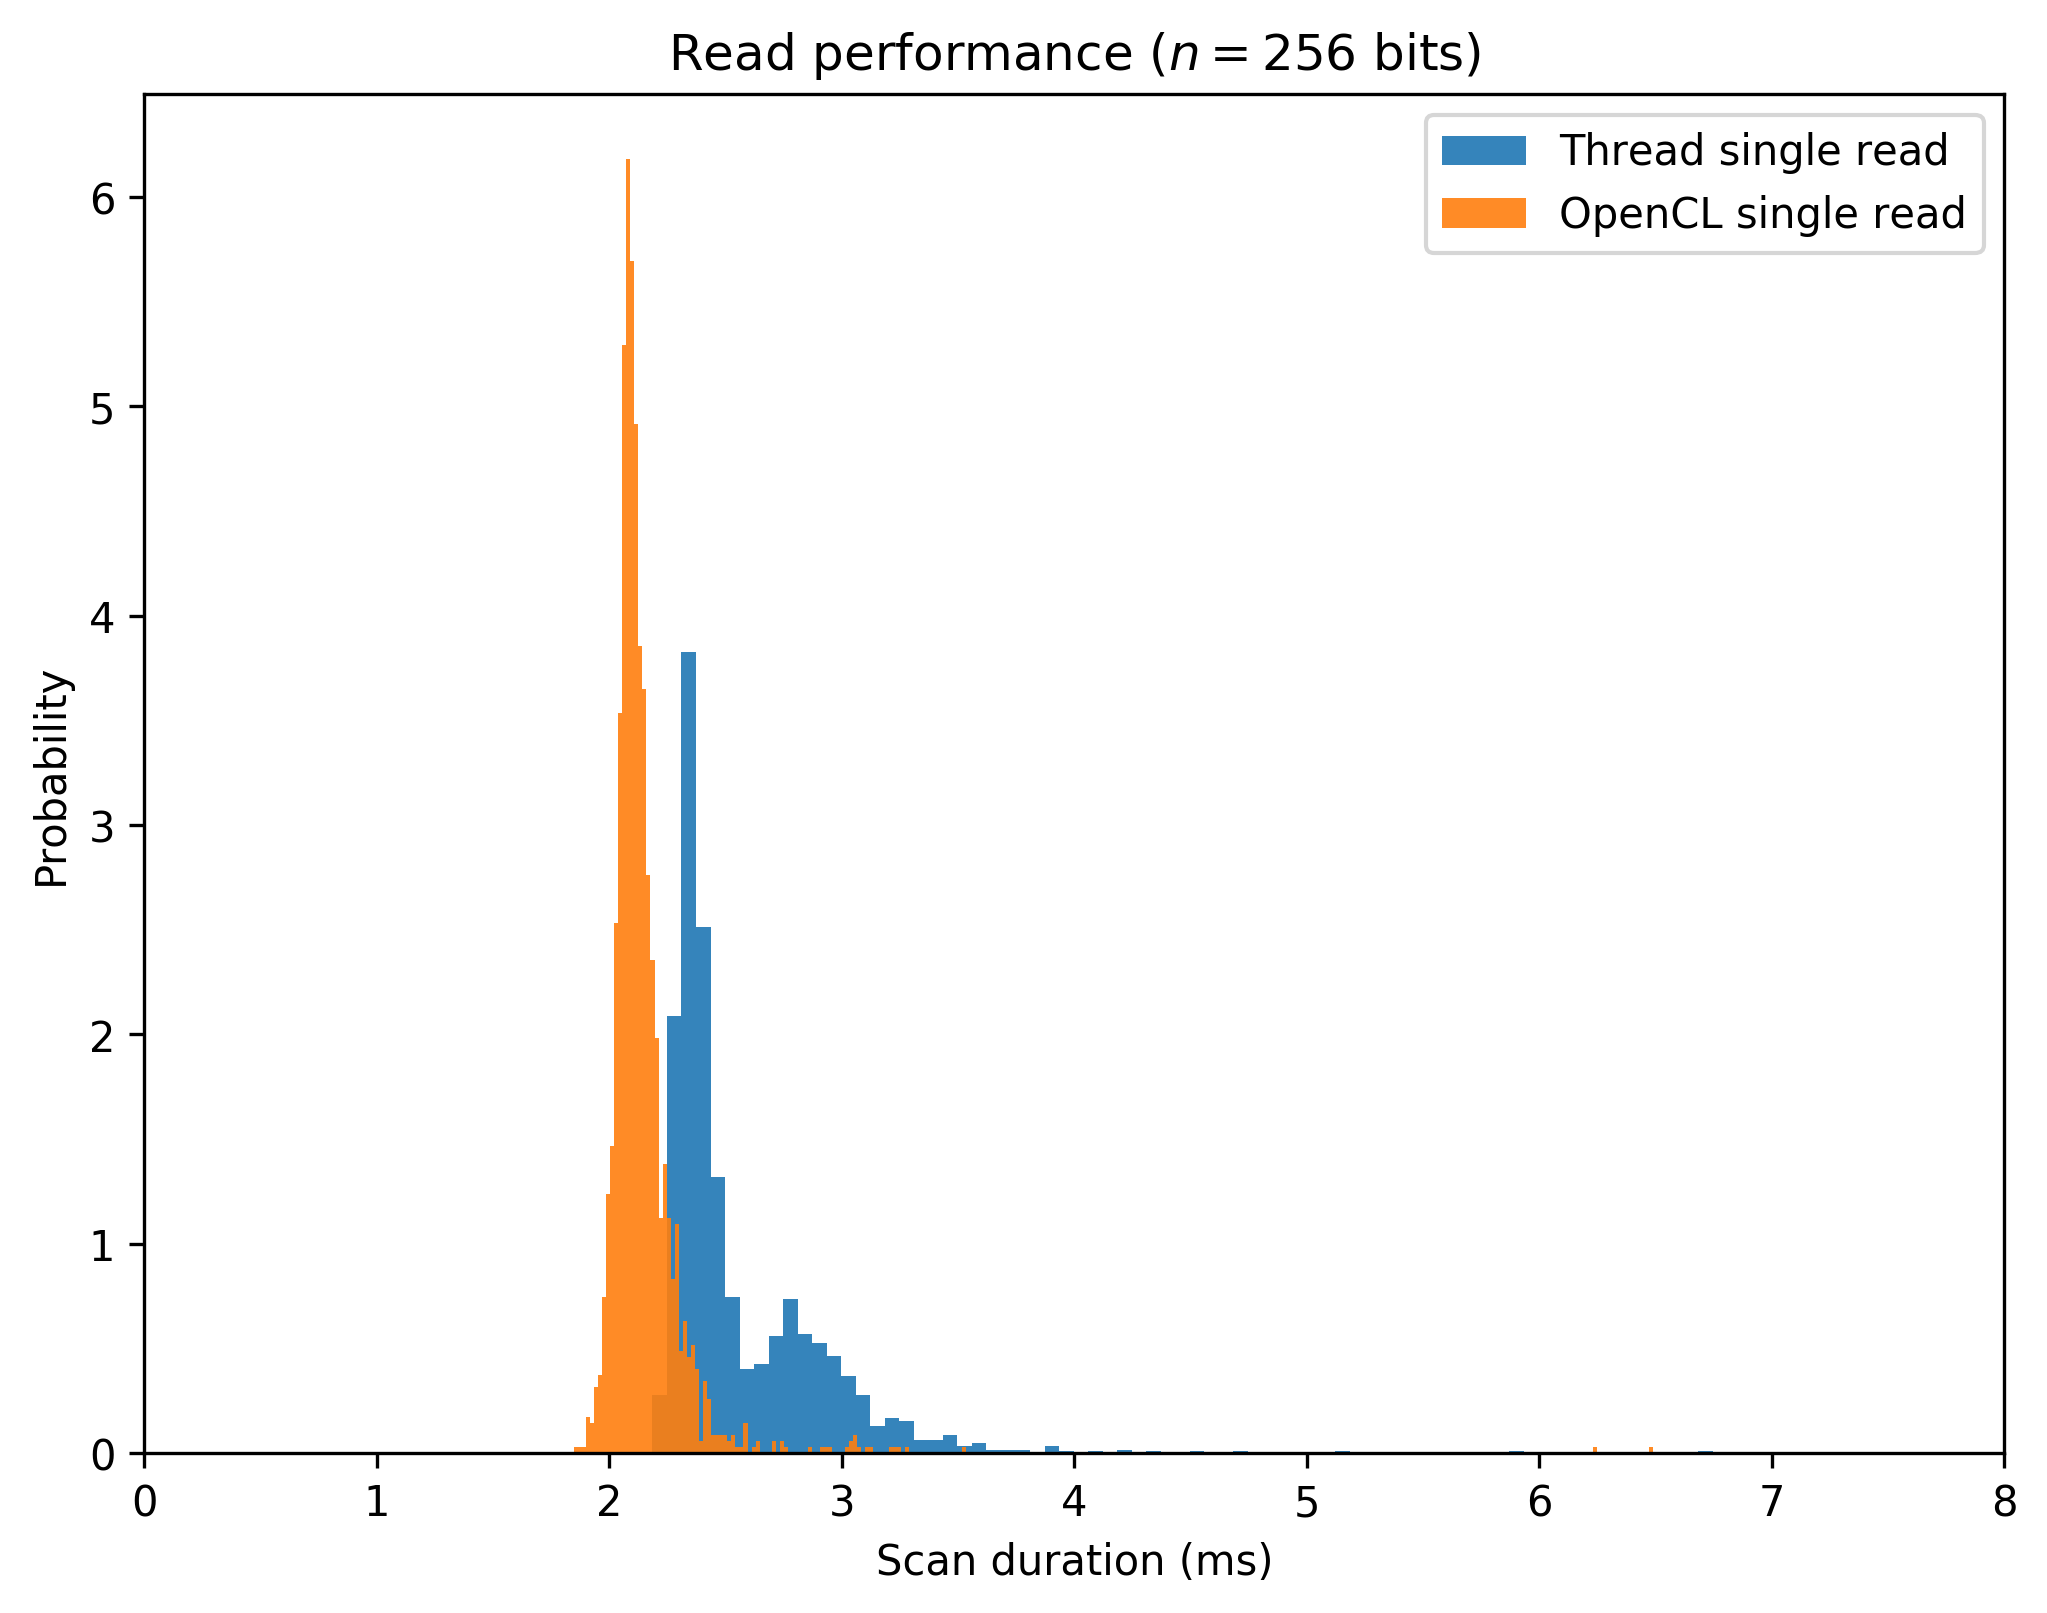
\includegraphics[width=\textwidth]{images02/performance/imac-read-256.png}
\caption{Time to run a single read in a SDM with $n=256$, $H=1,000,000$ and $r=103$.
\label{fig:perf-imac-read-256}}
\end{figure}

\begin{figure}[!htb]
\centering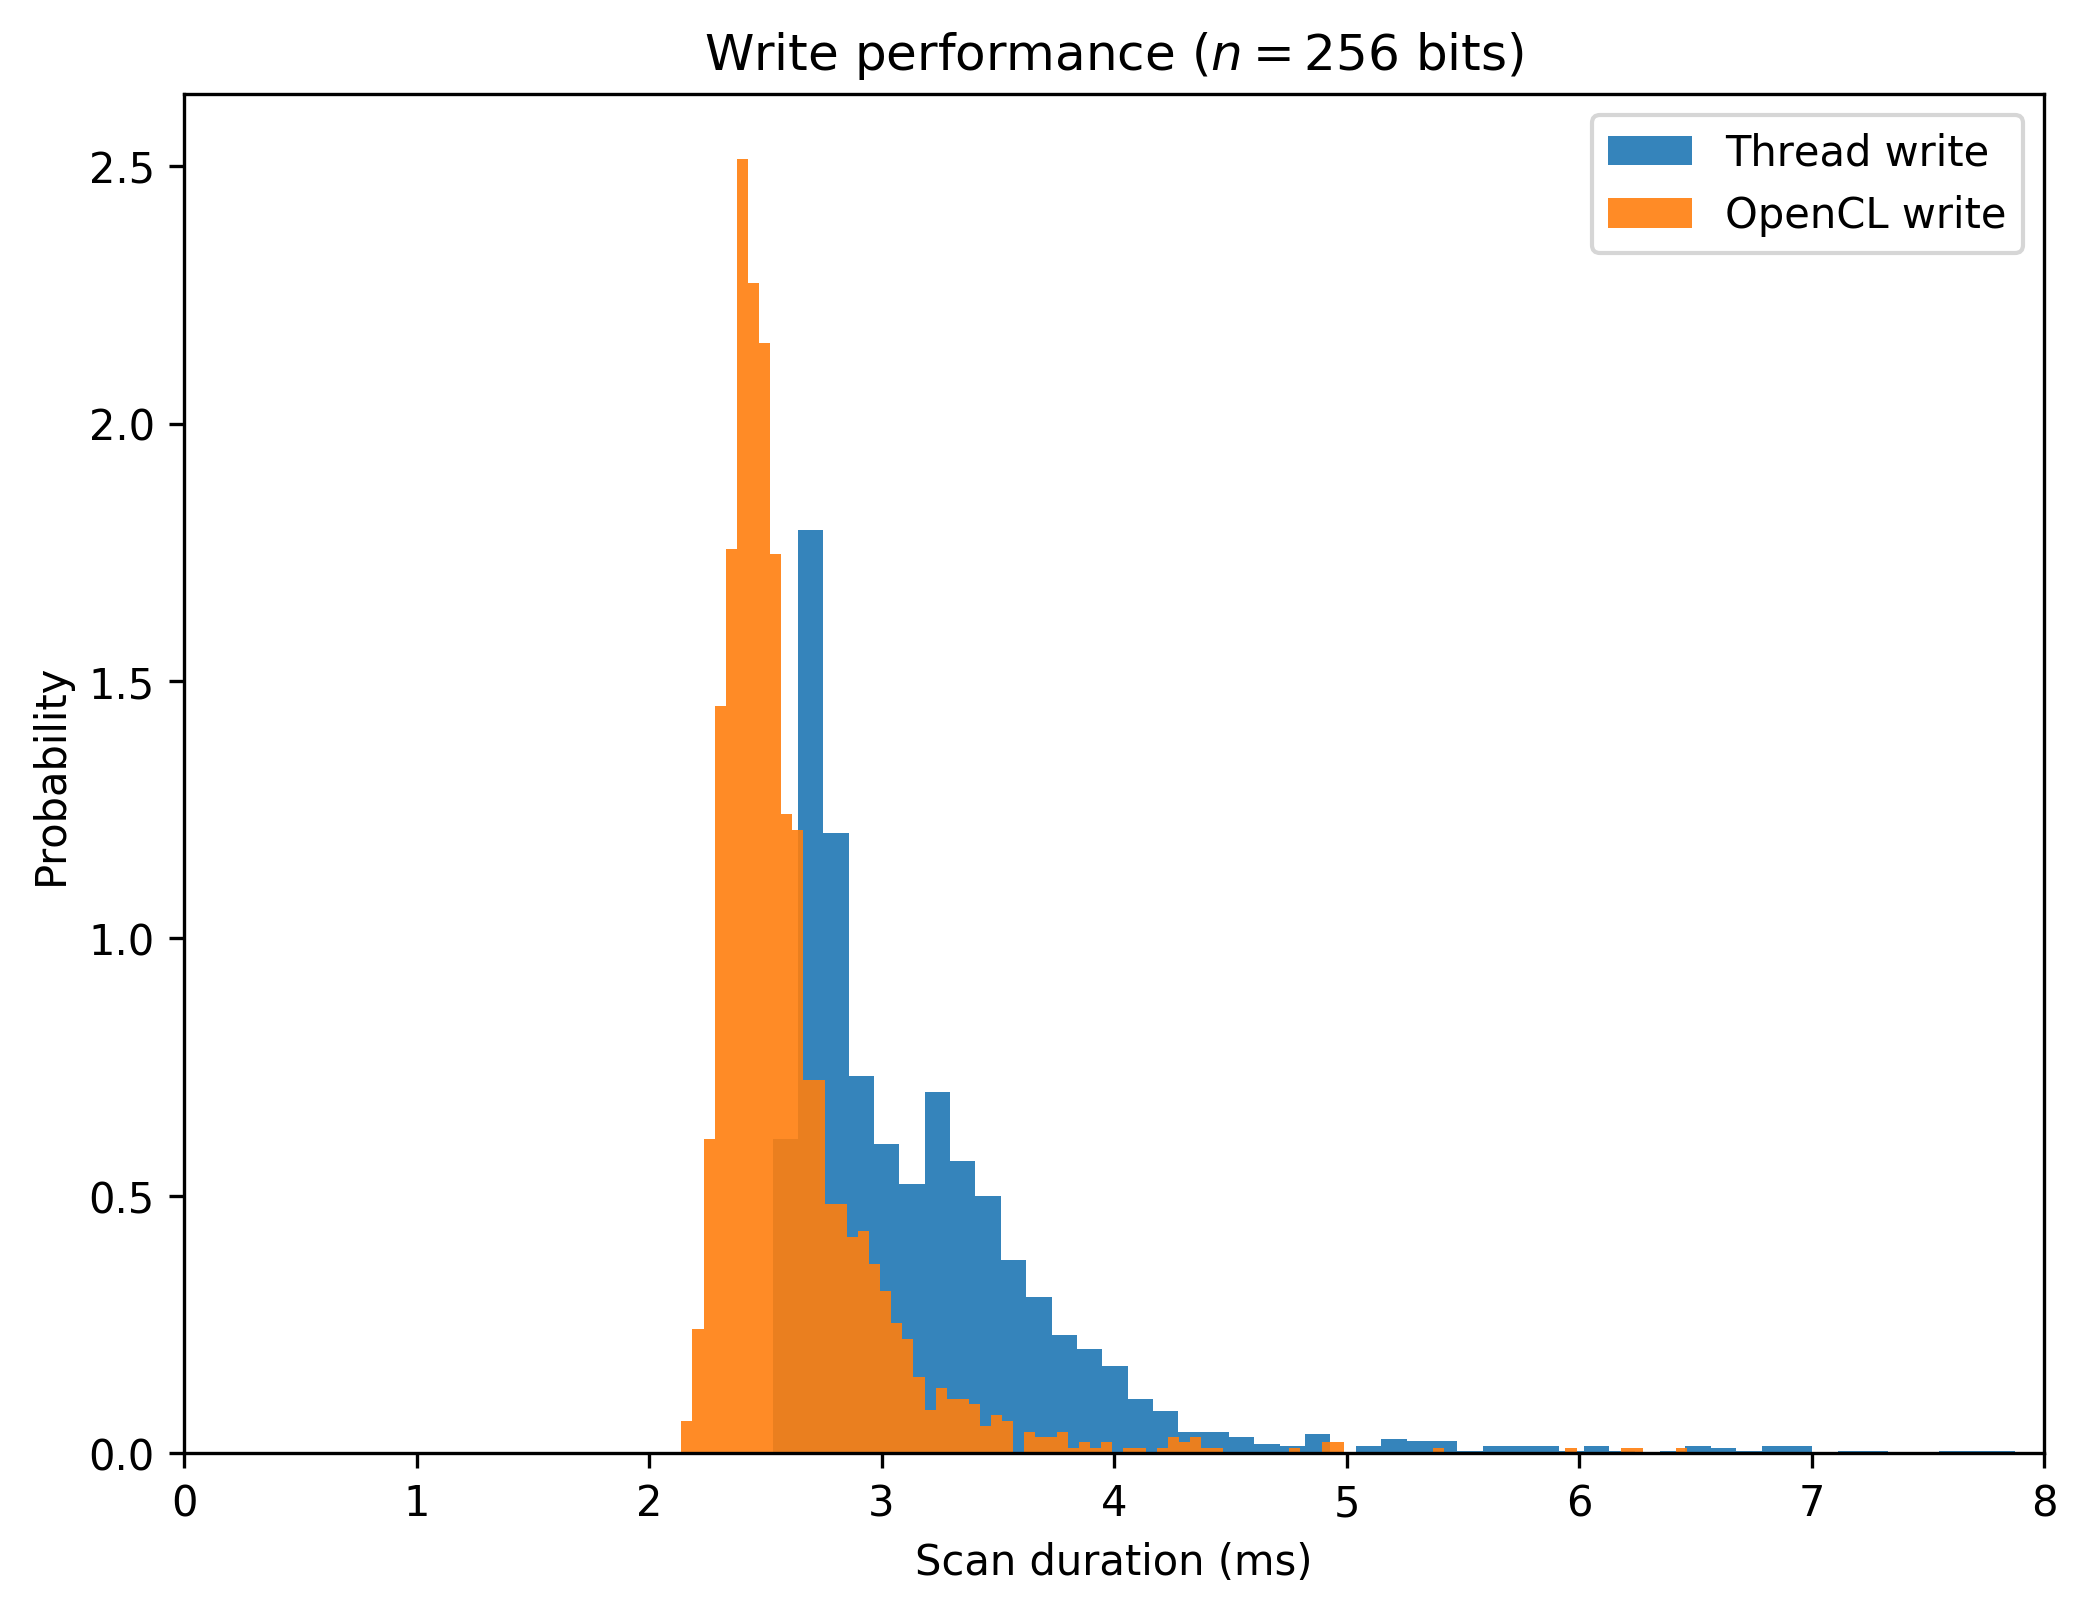
\includegraphics[width=\textwidth]{images02/performance/imac-write-256.png}
\caption{Time to run one write in a SDM with $n=256$, $H=1,000,000$ and $r=103$.
\label{fig:perf-imac-write-256}}
\end{figure}

\begin{figure}[!htb]
\centering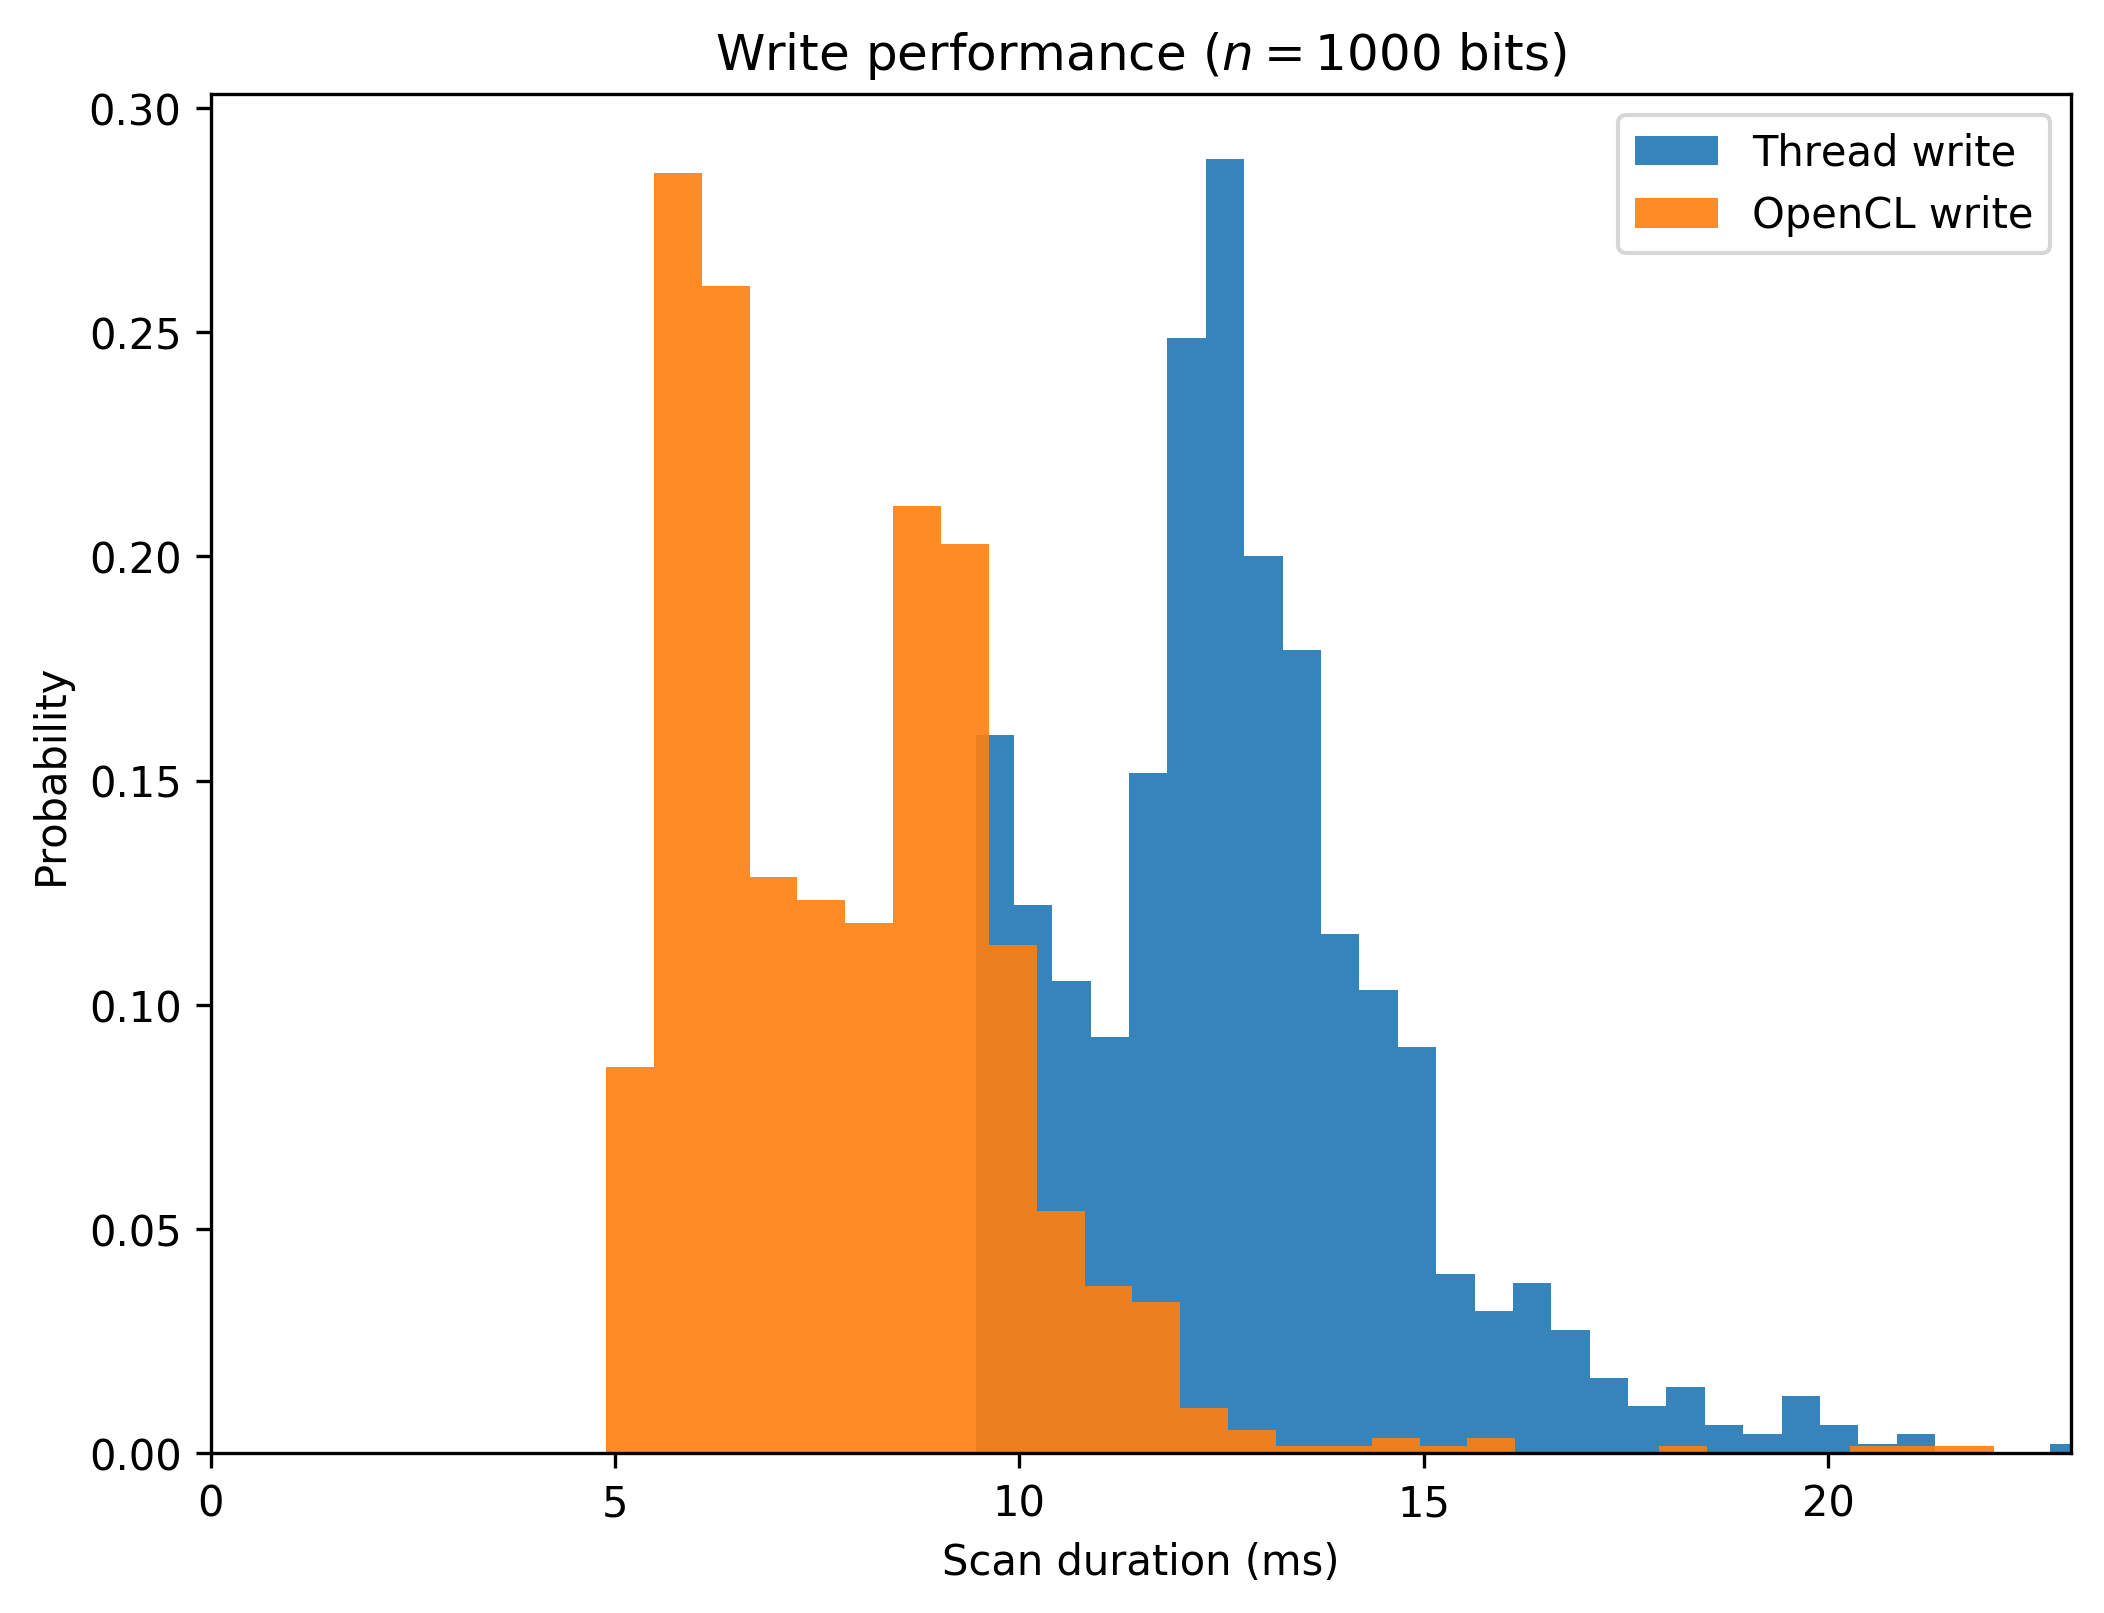
\includegraphics[width=\textwidth]{images02/performance/imac-write-1000.png}
\caption{Time to run one write in a SDM with $n=1,000$, $H=1,000,000$ and $r=451$.
\label{fig:perf-imac-write-1000}}
\end{figure}

\begin{figure}[!htb]
\centering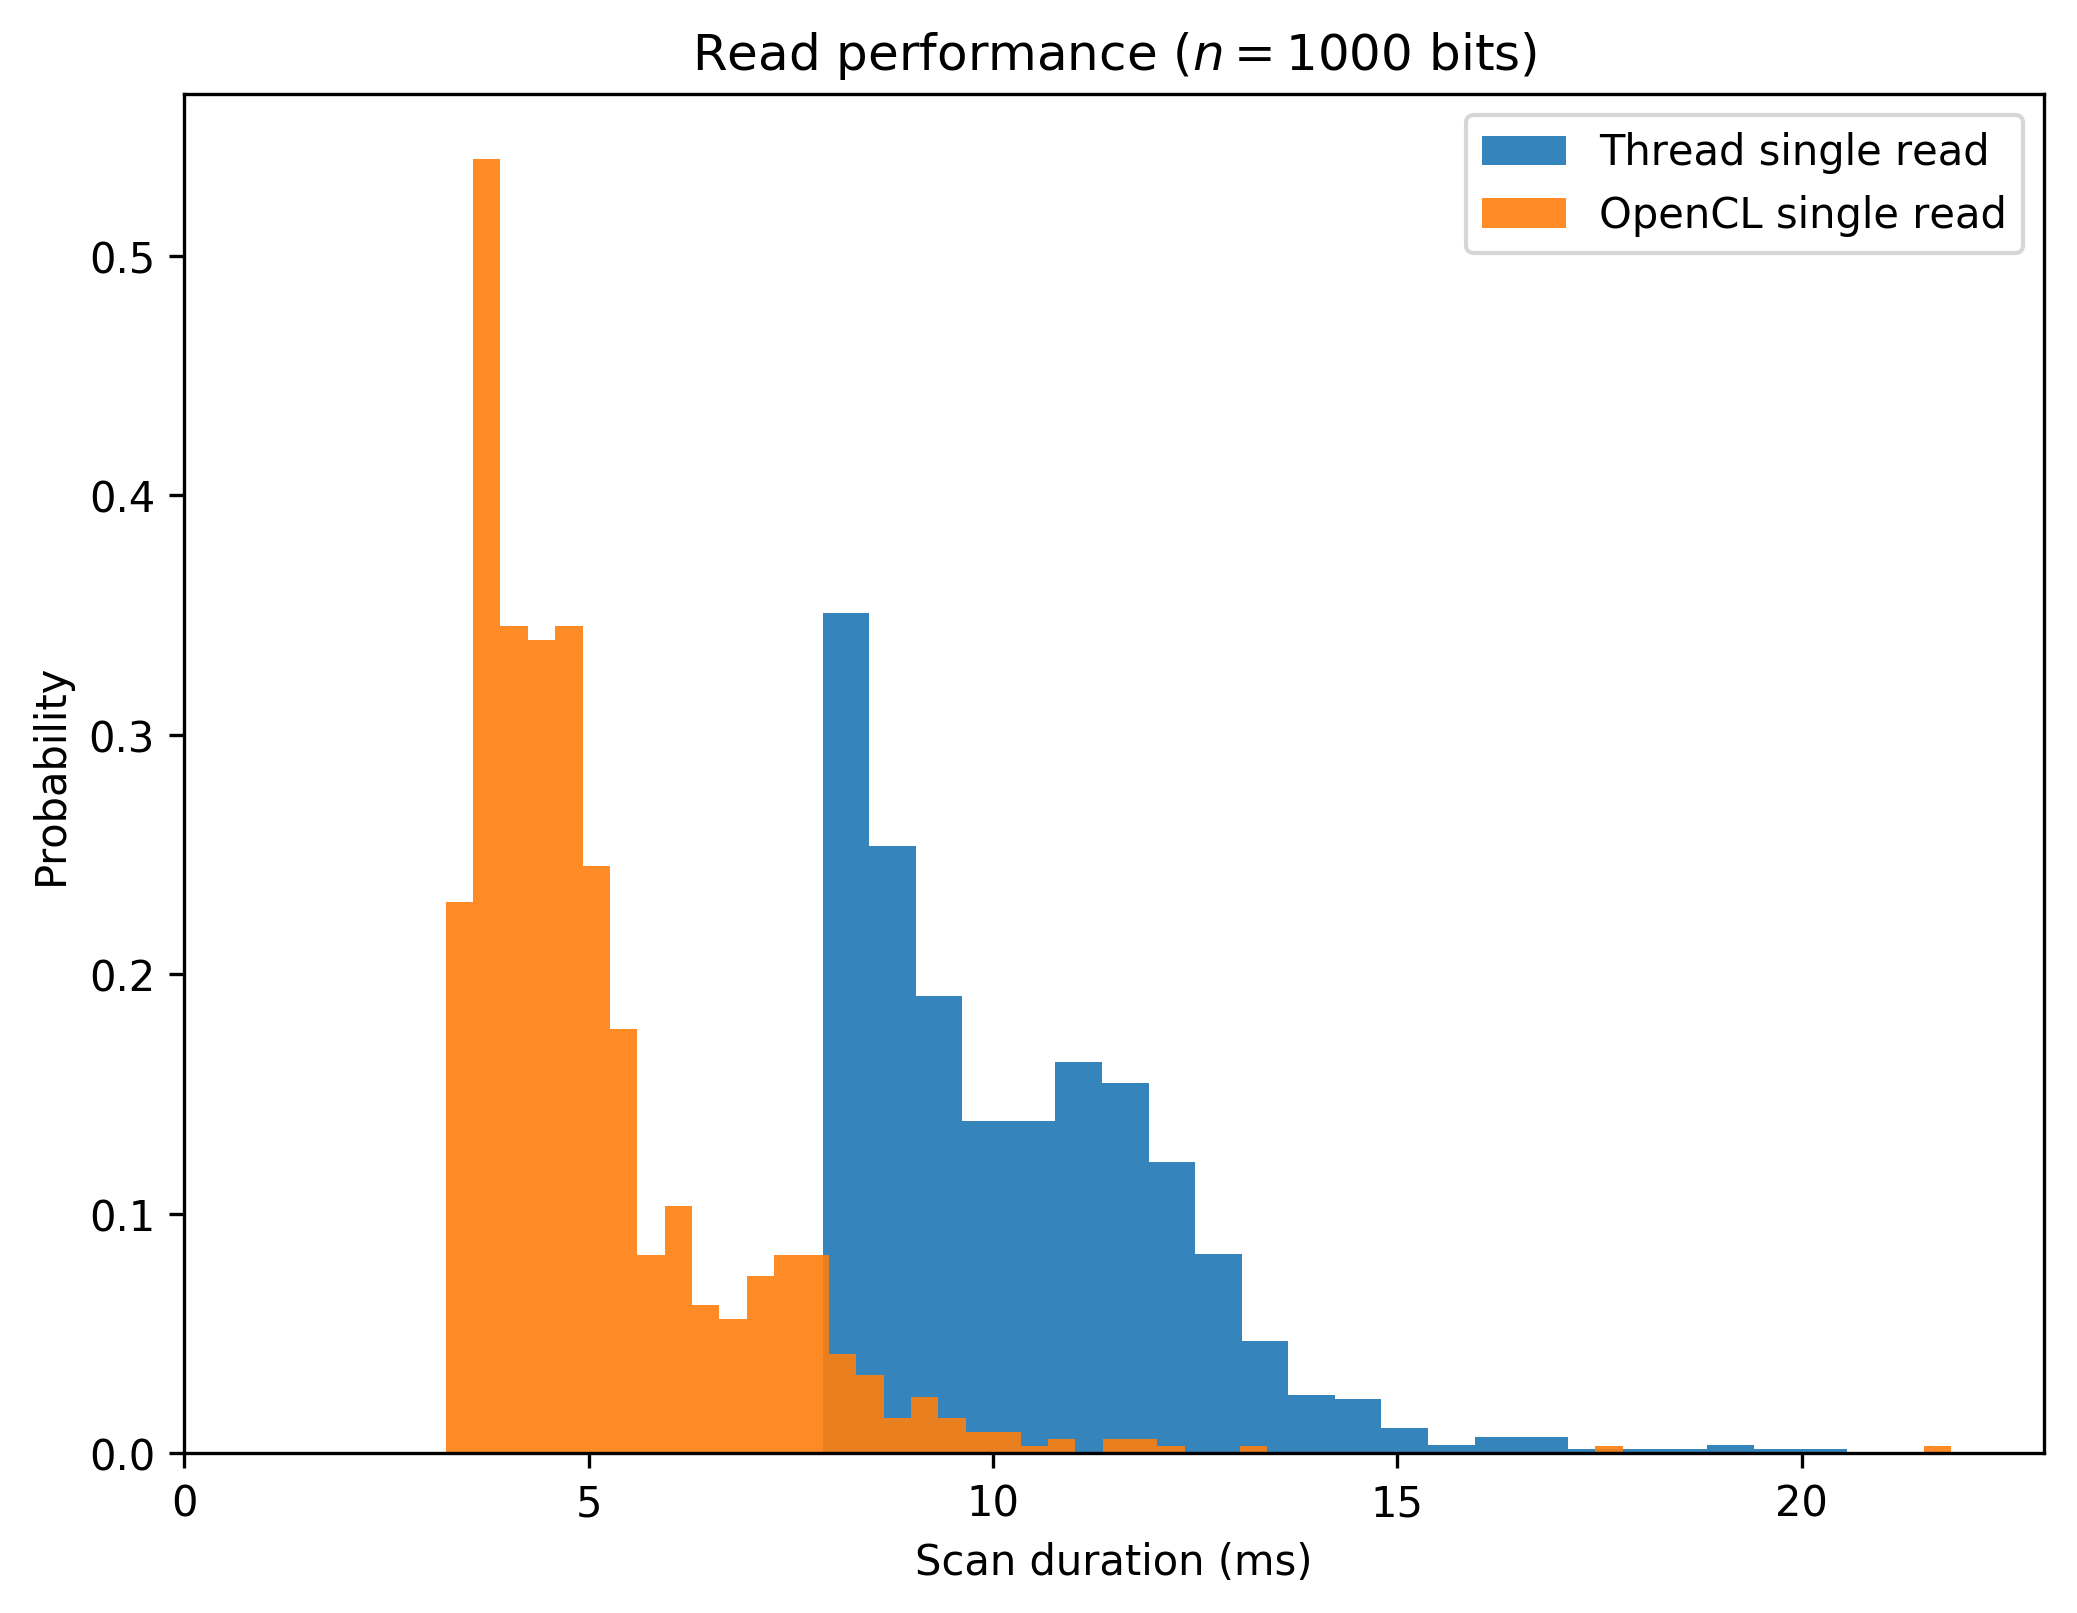
\includegraphics[width=\textwidth]{images02/performance/imac-read-1000.png}
\caption{Time to run a single read in a SDM with $n=1,000$, $H=1,000,000$ and $r=451$.
\label{fig:perf-imac-read-1000}}
\end{figure}

\begin{figure}[!htb]
\centering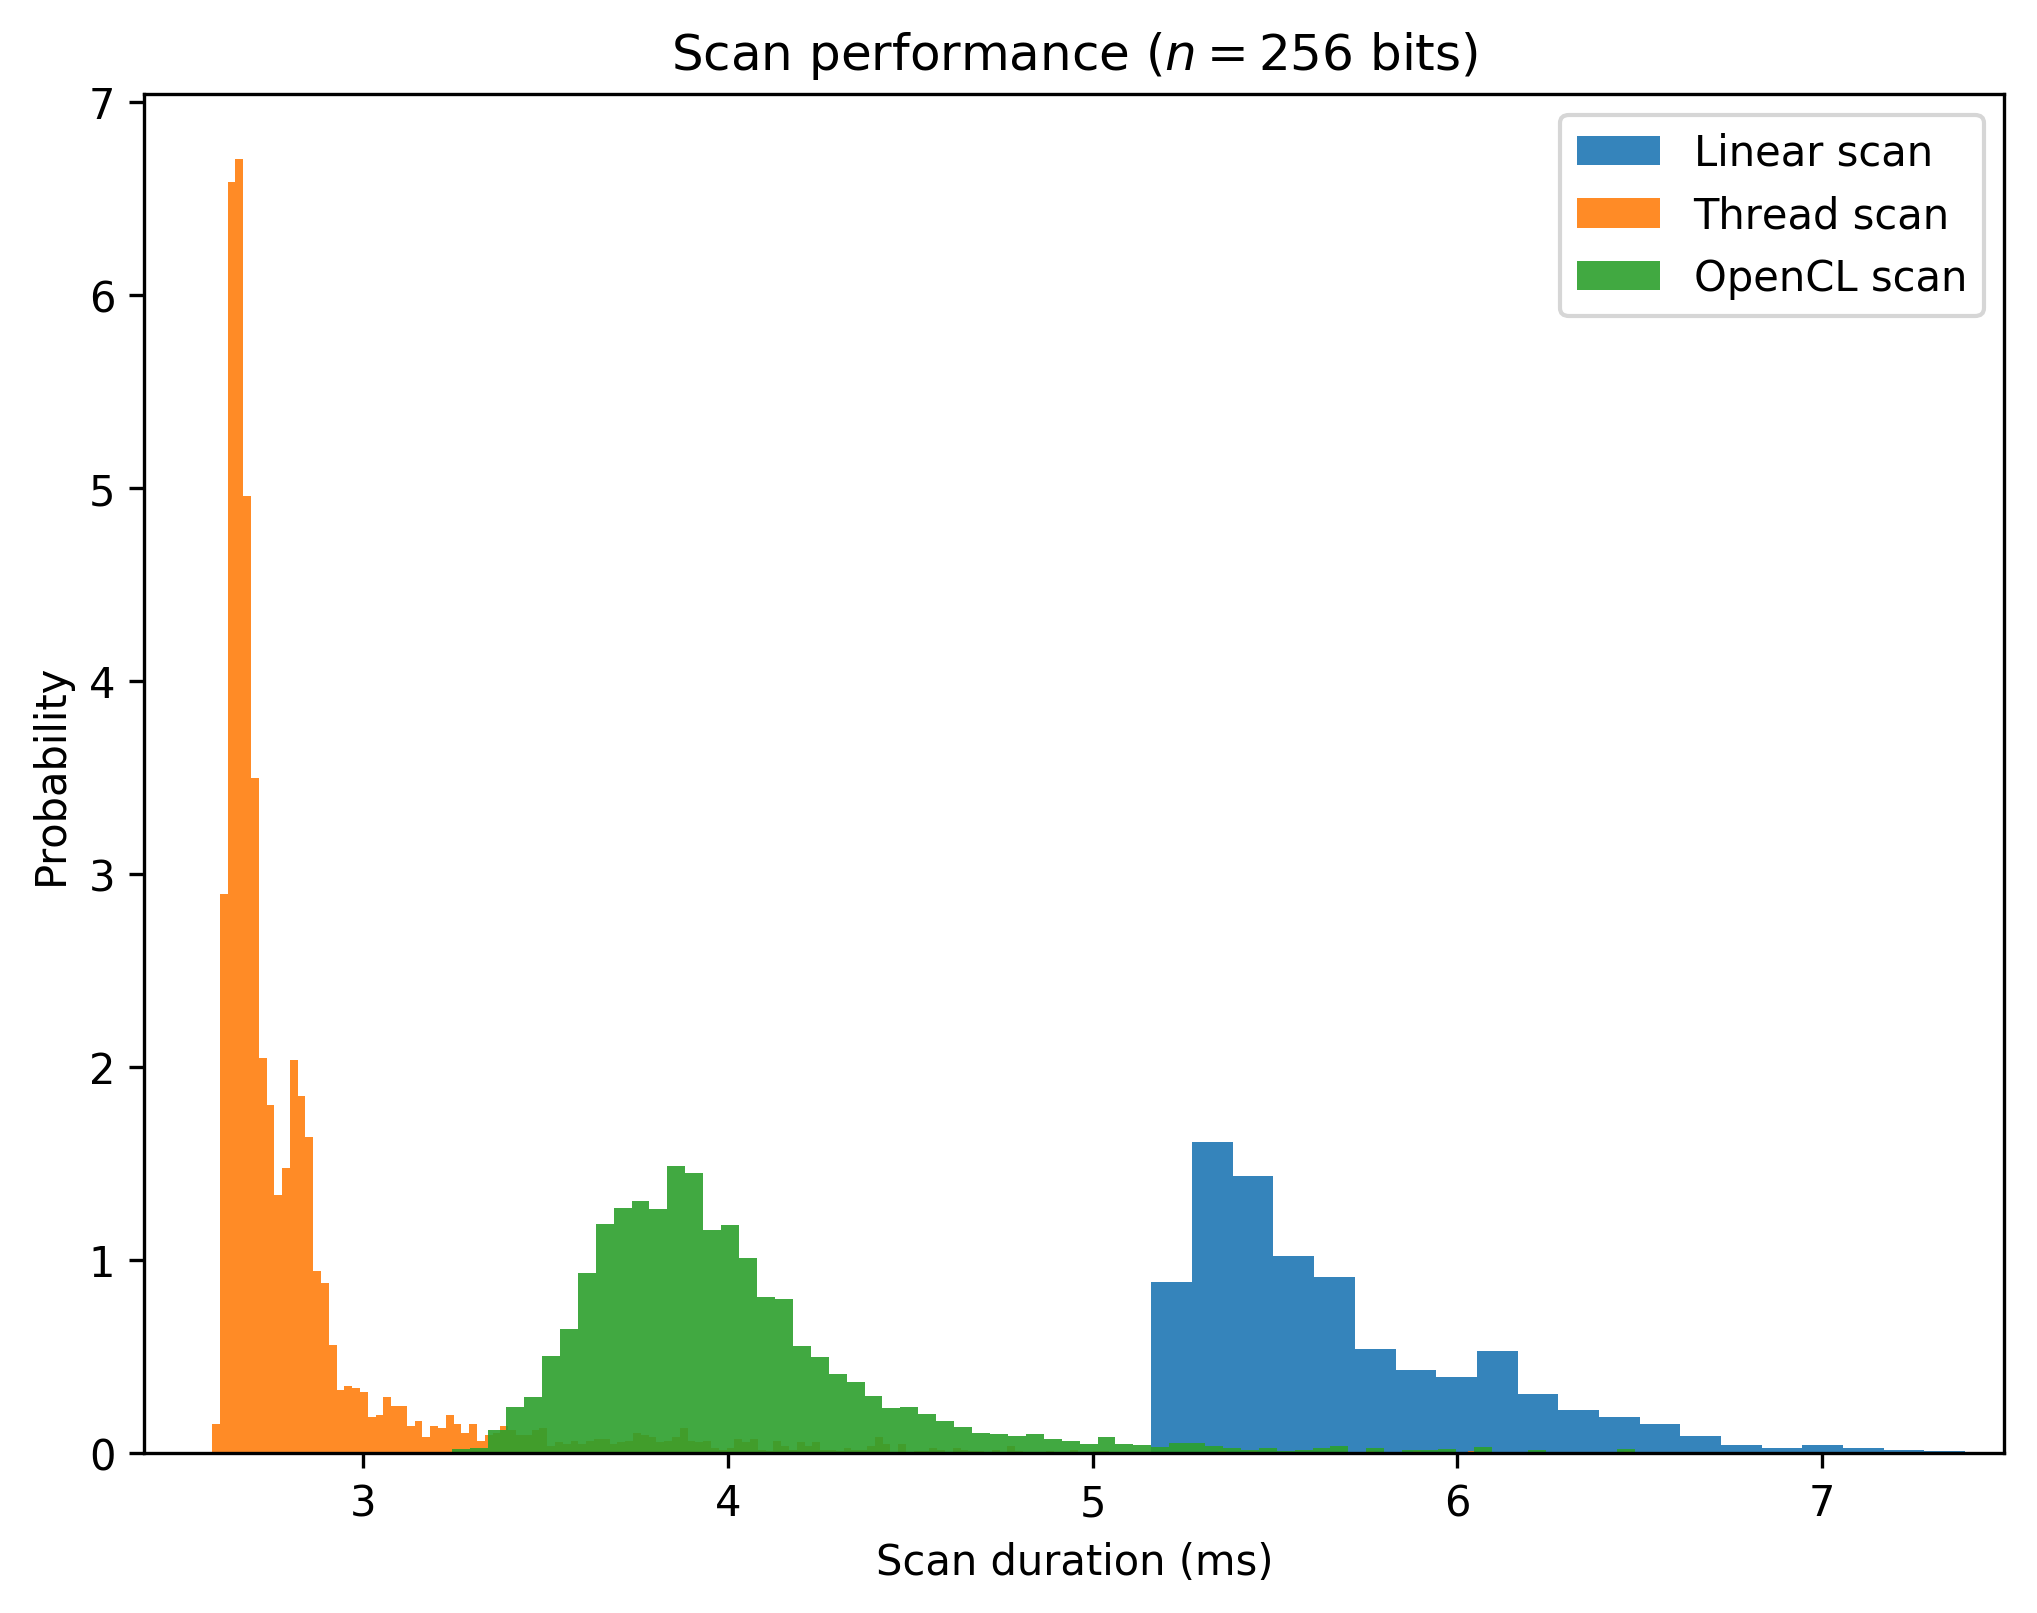
\includegraphics[width=\textwidth]{images02/performance/imac-scans-256.png}
\caption{Time to run a single scan in a SDM with $n=256$, $H=1,000,000$ and $r=103$.
\label{fig:perf-imac-scan-256}}
\end{figure}

\begin{figure}[!htb]
\centering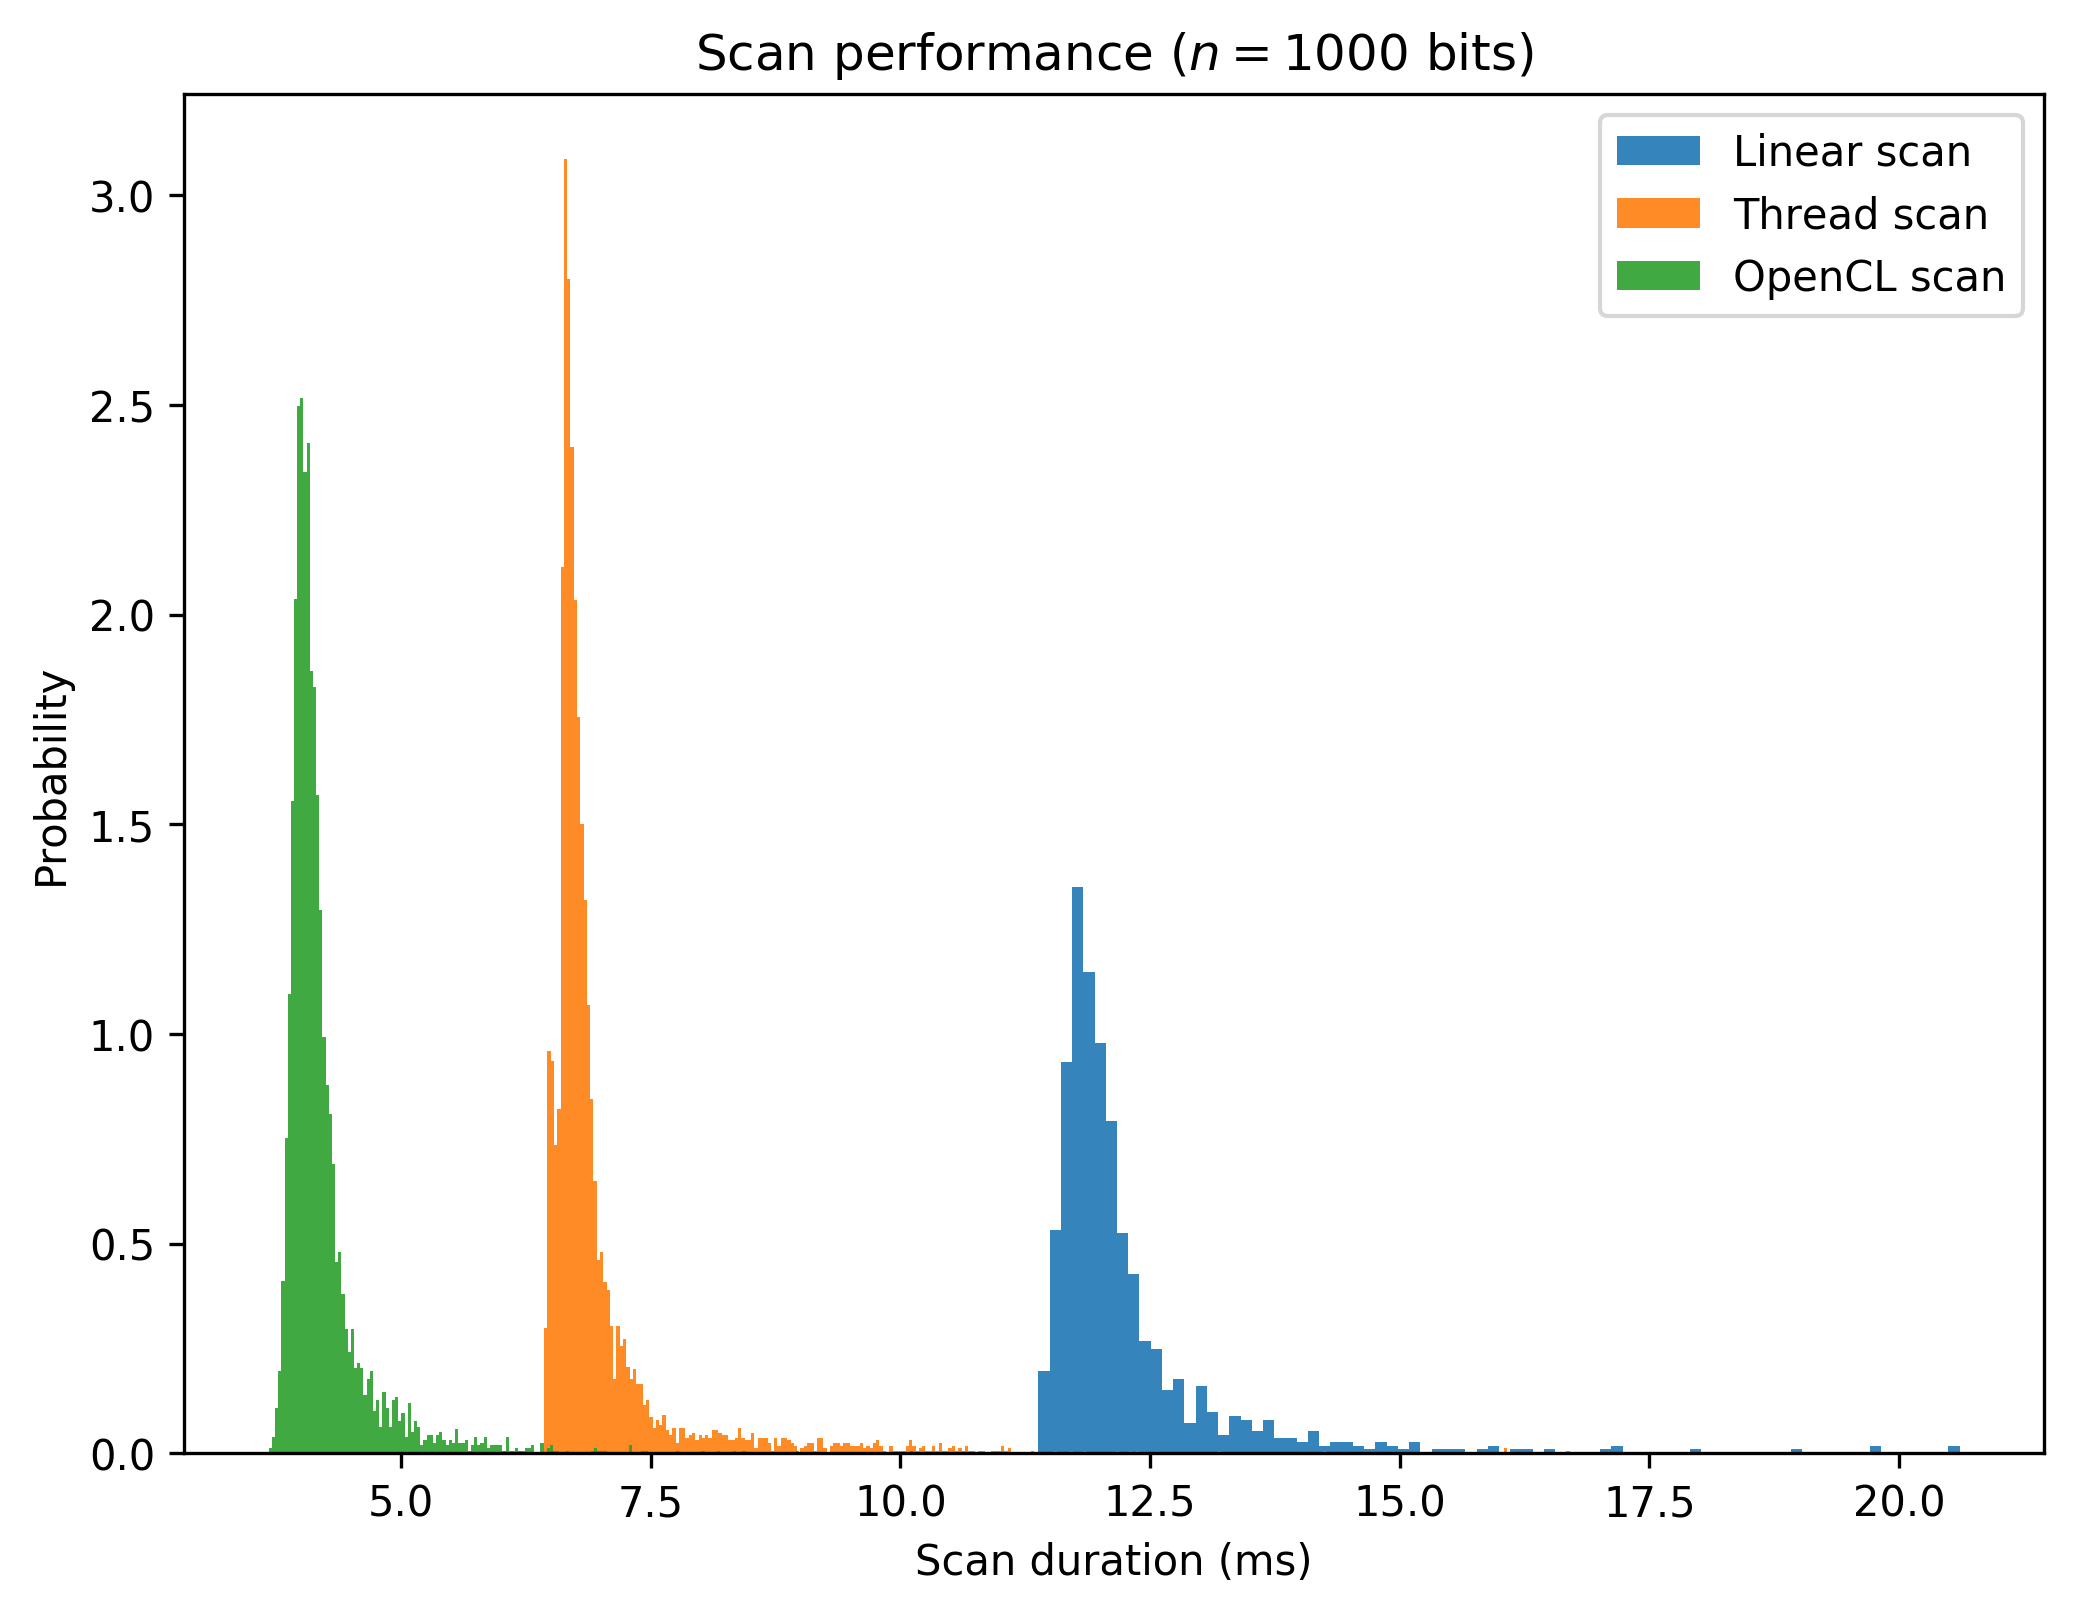
\includegraphics[width=\textwidth]{images02/performance/imac-scans-1000.png}
\caption{Time to run a single scan in a SDM with $n=1,000$, $H=1,000,000$ and $r=451$.
\label{fig:perf-imac-scan-1000}}
\end{figure}

\begin{figure}[!htb]
\centering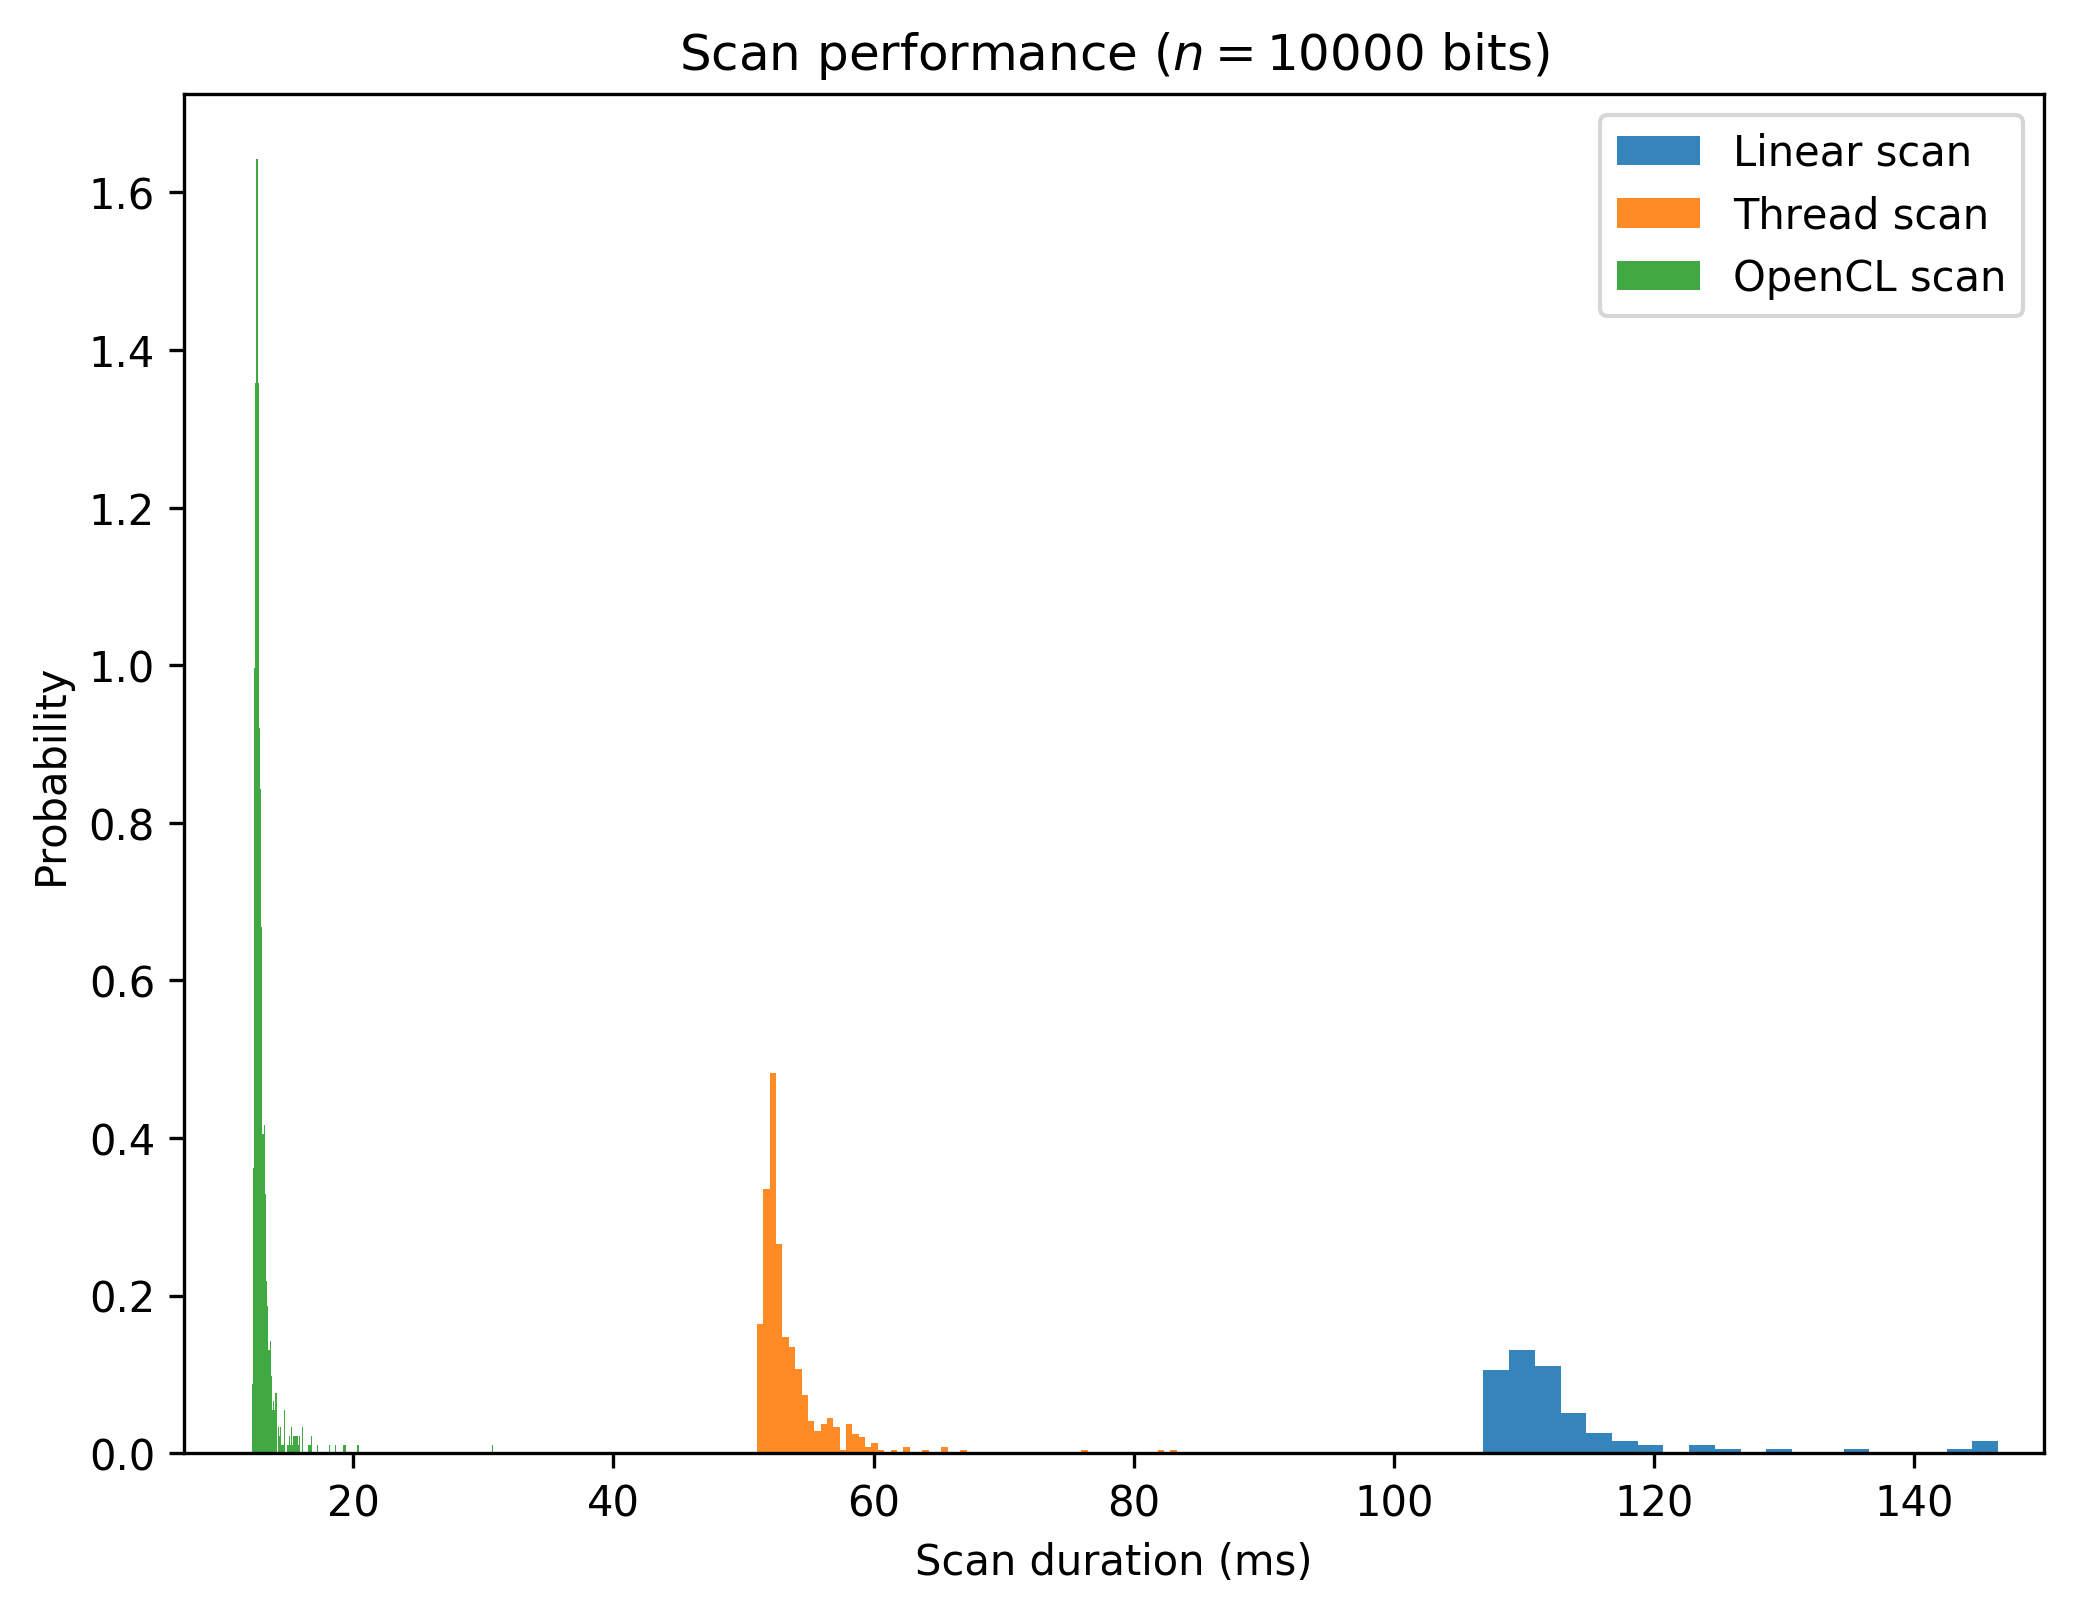
\includegraphics[width=\textwidth]{images02/performance/imac-scans-10k.png}
\caption{Time to run a single scan in a SDM with $n=10,000$, $H=1,000,000$ and $r=4845$.
\label{fig:perf-imac-scan-10k}}
\end{figure}

\begin{table}[!htb]
\centering
\begin{tabular}{| l | r | r | r |}
    \hline
    & Loops & Scans / second & Scan time (ms) \\ \hline
    Linear scan & 1000 & 81.62 & 12.25 \\
    Thread scan & 5000 & 143.68 & 6.95 \\
    OpenCL scan & 5000 & 238.00 & 4.20 \\ \hline
    \hline
    & Loops & Ops / second & Op. time (ms) \\ \hline
    Thread write & 1000 & 74.92 & 13.34 \\
    Thread single read & 1000 & 96.22 & 10.39 \\
    OpenCL write & 1000 & 126.50 & 7.90 \\
    OpenCL single read & 1000 & 190.20 & 5.25 \\
    \hline
\end{tabular}
\caption{iMac Retina 5K 27-inch 2017 with a 3.8GHz Intel core i5 processor, 8GB DDR4 RAM, and a Radeon Pro 580 8G GPU. Running an SDM with $n=1,000$ bits, $H=1,000,000$, and $r=451$.
\label{tab:perf-imac-1000}}
\end{table}

\begin{table}[!htb]
\centering
\begin{tabular}{| l | r | r | r |}
    \hline
    & Loops & Scans / second & Scan time (ms) \\ \hline
    Linear scan & 1000 & 175.48 & 5.69 \\
    Thread scan & 5000 & 352.63 & 2.83 \\
    OpenCL scan & 5000 & 244.88 & 4.08 \\ \hline
    \hline
    & Loops & Ops / second & Op. time (ms) \\ \hline
    Thread write & 2000 & 304.46 & 3.28 \\
    Thread single read & 2000 & 391.21 & 2.55 \\
    OpenCL write & 2000 & 378.44 & 2.64 \\
    OpenCL single read & 2000 & 466.16 & 2.14 \\
    \hline
\end{tabular}
\caption{iMac Retina 5K 27-inch 2017 with a 3.8GHz Intel core i5 processor, 8GB DDR4 RAM, and a Radeon Pro 580 8G GPU. Running an SDM with $n=256$ bits, $H=1,000,000$, and $r=103$.
\label{tab:perf-imac-256}}
\end{table}

\begin{table}[!htb]
\centering
\begin{tabular}{| l | r | r | r |}
    \hline
    & Loops & Scans / second & Scan time (ms) \\ \hline
    Linear scan & 100 & 8.59 & 116.38 \\
    Thread scan & 500 & 18.66 & 53.56 \\
    OpenCL scan & 1000 & 77.20 & 12.95 \\
    \hline
\end{tabular}
\caption{iMac Retina 5K 27-inch 2017 with a 3.8GHz Intel core i5 processor, 8GB DDR4 RAM, and a Radeon Pro 580 8G GPU. Running an SDM with $n=10,000$ bits, $H=1,000,000$, and $r=4845$.  There is no benchmark for read and write operations because RAM is not enough to allocate the counters --- it would consume 37.25 GB of RAM.
\label{tab:perf-imac-10k}}
\end{table}
